\documentclass[11pt, oneside]{article} 
\usepackage{geometry}
\geometry{letterpaper} 
\usepackage{graphicx}
	
\usepackage{amssymb}
\usepackage{amsmath}
\usepackage{parskip}
\usepackage{color}
\usepackage{hyperref}

\graphicspath{{/Users/telliott/Dropbox/Github-Math/quickgeo/figures/}{/Users/telliott/Dropbox/Github-Math/figures/}}
% \begin{center} \includegraphics [scale=0.4] {gauss3.png} \end{center}

\title{Constructs}
\date{}

\begin{document}
\maketitle
\Large

%[my-super-duper-separator]

\subsection*{equilateral triangle}

The first figure shows how to construct an equilateral triangle with straight-edge and compass.  (A straight-edge is a ruler with no rules, no marked divisions).

Pick a base of the desired length.  Then using one end of the base as the center of a circle, draw the circle of radius equal to the length of the base.  (i.e. set the compass to the base length).
\begin{center} 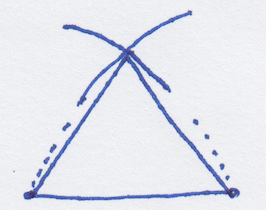
\includegraphics [scale=0.8] {H1.png} \end{center}

We're only showing the part of the arc that matters.  Repeat using the other point.  Where the arcs cross, we have a point that is the same distance from each end of the original base, and that distance is equal to the base, so together with the ends of the base, this point forms one of the vertices of an equilateral triangle.
\begin{center} 
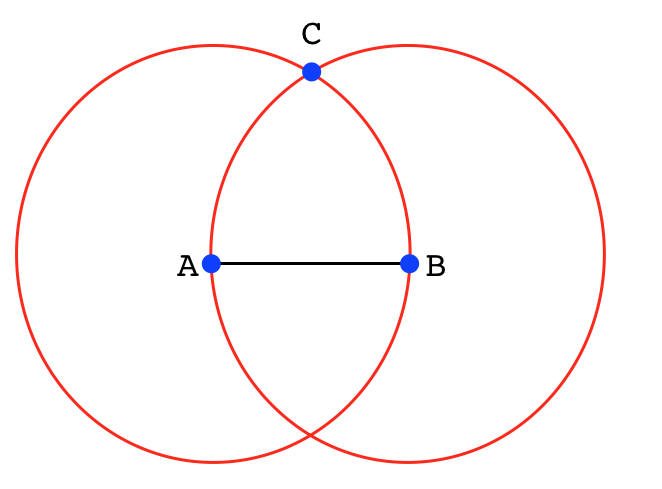
\includegraphics [scale=0.20] {PI_1b.png} 
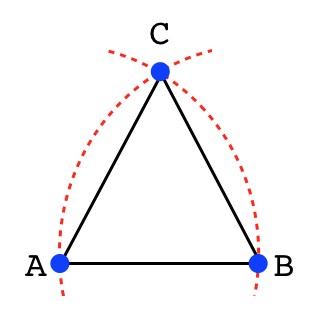
\includegraphics [scale=0.25] {PI_1c.png} 
\end{center}

\subsection*{perpendicular bisector}

There are three different cases:

$\circ$ \ (1) A perpendicular bisector at a point on a line.

$\circ$ \ (2) A perpendicular bisector through a line, midway between two other points.

$\circ$ \ (3) A perpendicular through a line and an external point.

Let us solve the second one first.  Draw two circles to form two equilateral triangles above and below the line.
\begin{center} 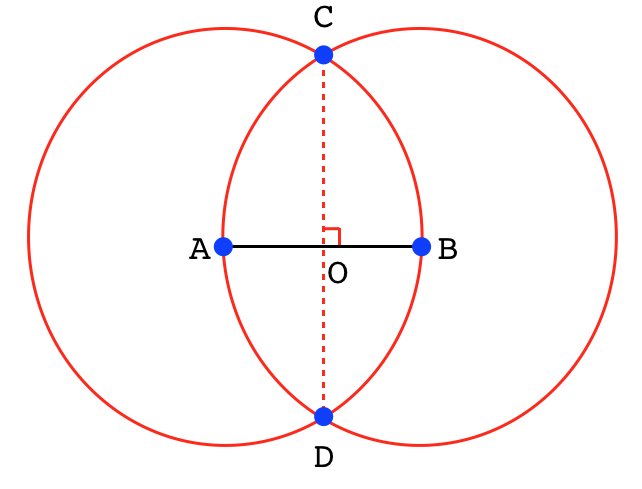
\includegraphics [scale=0.25] {PI_1d.png} \end{center}
Draw the line $CD$ connecting the apex of the first triangle with that of the second triangle below.  I claim that the angles at $O$ are all right angles and $AB$ is bisected.

\emph{Proof}.

\begin{center} 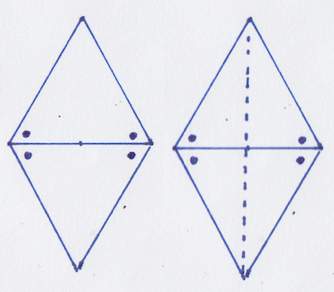
\includegraphics [scale=0.5] {H19.png} \end{center}
In the left panel, we have two triangles congruent by ASA (or SSS or SAS, take your pick).  All five lines in the figure are equal length, and all angles are equal as well (the top and bottom aren't marked).

The two triangles formed by the dotted line (right panel) are congruent by SAS, so the top and bottom angles are bisected.  Therefore, all four small triangles are congruent, by ASA.

It follows from the congruent triangles that $\angle AOC = \angle BOC$ so they are both right angles, and then all the angles at $O$ are right angles and $AB$ is bisected at $O$.

$\square$

The other two cases can be converted into the second.  For the first, draw a circle around the given point, smaller than the radius to be used for the equilateral triangles.  That circle will cross the line at two points equidistant from the given point.  Proceed with case 2.
\begin{center} 
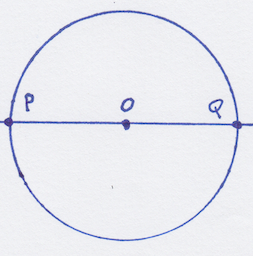
\includegraphics [scale=0.4] {H17.png} 
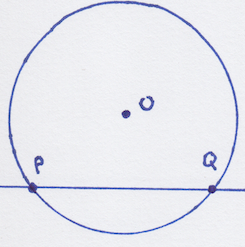
\includegraphics [scale=0.4] {H18.png} 
\end{center}
For the third case, draw a circle around the external point, to find two points on the line that are equidistant from the given point and so form an isosceles triangle with it.  Proceed with case 2 as before. 

Points on the perpendicular bisector are equidistant from the points $A$ and $B$.  Examples:  $P$ has $PA = PB$ and $Q$ has $QA = QB$.  This is true of every point on the vertical line (figure below).
\begin{center} 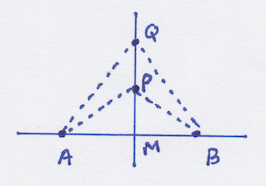
\includegraphics [scale=0.6] {H4.png} \end{center}

\subsection*{circle containing any three points}

Next, for any three points, we can draw a circle that contains those points.  Consider first the points $A$, $B$ and $C$ in the figure below.  Draw $AB$ and its perpendicular bisector.  Draw $BC$ and its perpendicular bisector.  The point where they cross is $O$, the center of the circle containing all three points.

\emph{Proof}.
All the points on the first bisector are equidistant from $A$ and $B$, and on the second, equidistant from $B$ and $C$.  Hence $AO = BO = CO$.

\begin{center} 
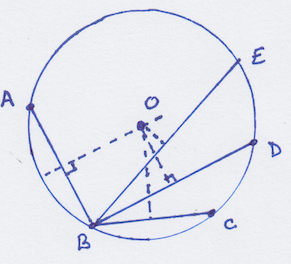
\includegraphics [scale=0.5] {H3c.png} 
\end{center}

The point where the bisectors meet is equidistant from all three points.  Therefore it can be used as the center for a circle that contains all three of them.

For any other point on the circle, such as $D$ or $E$, the perpendicular bisector has the same property.  Hence they all go through point $O$.

\subsection*{angle bisection}

Next, we will bisect an angle.  A method is shown here:
\begin{center} 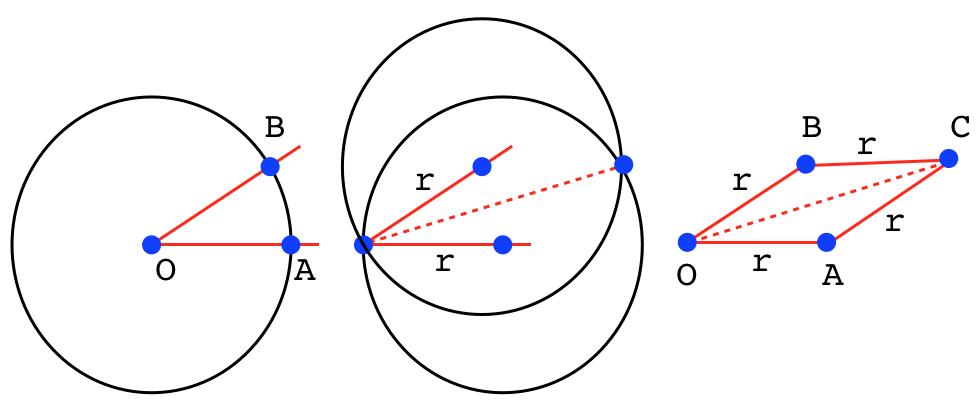
\includegraphics [scale=0.4] {PI_9a.png} \end{center}  
Suppose we wish to bisect the angle at vertex $O$.  Mark off $OA = OB$.  Draw two circles with the same radius, whose arcs are shown meeting at $C$.  We have that $AC = BC$.  

By the isosceles triangle theorem, $\angle OBA = \angle OAB$ and $\angle ABC = \angle BAC$ so their sums, namely the total $\angle OBC = \angle OAC$.  Now we have SAS.

Therefore, $\triangle OBC \cong \triangle OAC$.  So the two angles at $O$, $\angle BOC$ and $\angle AOC$, are equal.

\subsection*{tangent}

At each point where the radius intersects the circle, we can draw the tangent to the circle at that point.
\begin{center} 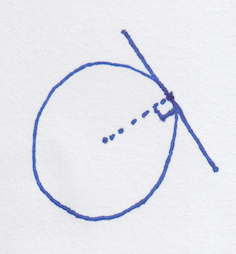
\includegraphics [scale=1.] {H5.png} \end{center}

One way to do this is to extend the radius the same length again and draw its perpendicular bisector.  

On the other hand, if we want the tangent to go through a particular exterior point $P$, connect the center of the circle $O$ to that point, then bisect the resulting length at $M$.  

\begin{center} 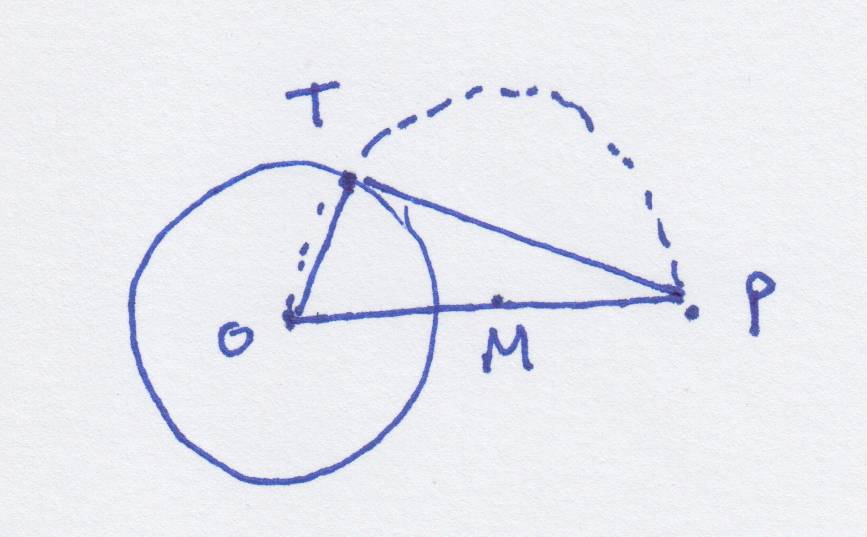
\includegraphics [scale=1.0] {H5b.png} \end{center}

A circle drawn with length $OM$ and its center at the bisection point will form a right angle at the point $T$ where it intersects the circle.  This follows from Thales circle theorem.




\end{document}